\documentclass{standalone}
\usepackage{tikz}
\usepackage{ctex,siunitx}
\setCJKmainfont{Noto Serif CJK SC}
\usepackage{tkz-euclide}
\usepackage{amsmath}
\usetikzlibrary{patterns, calc,3d}
\usetikzlibrary {decorations.pathmorphing,decorations.pathreplacing,decorations.shapes}
\tikzset{label style/.append style={font=\small}}
\begin{document}
\small
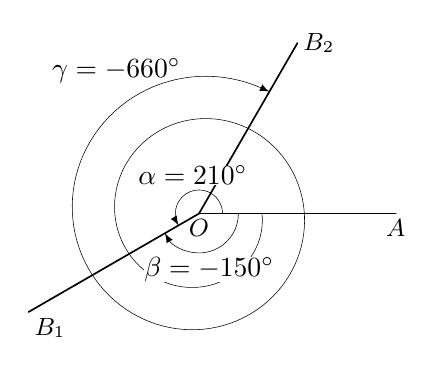
\begin{tikzpicture}[>=latex,scale=1.0,inner sep=2pt]
  \tkzDefPoints{0/0/O,2.5/0/A}
  \tkzDefPoint(60:2.5){B2}
  \tkzDefPoint(-150:2.5){B1}
  \tkzDrawSegments[semithick](O,A O,B2 O,B1)
  \tkzLabelPoints(A,O)
  \tkzLabelPoint[right](B2){$B_2$}
  \tkzLabelPoint[below right](B1){$B_1$}
  \draw[very thin,->,samples=200,domain=0:-660]plot(\x:{0.8-\x*0.0015});
  \draw[very thin,->](0.3,0)arc(0:210:0.3)node[midway,above=2pt,inner sep=0pt,fill=white]{$\alpha=\ang{210}$};
  \draw[very thin,->](0.5,0)arc(0:-150:0.5)node[midway,below=2pt,inner sep=0pt,fill=white]{$\beta=\ang{-150}$};
\node at (120:2.1){$\gamma=-\ang{660}$};
\end{tikzpicture}
\end{document}